%---------------DOCUMENT SETTINGS------------------------------------
%\documentclass[headheight=30pt]{scrartcl}
\documentclass{article}

\usepackage[utf8]{inputenc} % utf8x durch utf8 ersetzt wegen biblatex
\usepackage[T1]{fontenc}
\usepackage{amsmath,amssymb,amstext,amsfonts}
\usepackage[ngerman]{babel}
\usepackage{csquotes}
\usepackage{pdfpages} %zum importieren des Deckblattes
\usepackage{geometry}
\usepackage[headsepline]{scrlayer-scrpage}
\usepackage{lastpage}
\usepackage[style=numeric]{biblatex} %Literaturverwaltung
\usepackage{tabularx} %für die Legende im Gruundlagen Oszi Bild
\usepackage{float}
\usepackage{textcomp}
\usepackage{gensymb}
\usepackage{stmaryrd}
\usepackage{graphicx}
\usepackage[export]{adjustbox}
\usepackage{a4wide}
\usepackage{hyperref}
\usepackage{multicol}
\usepackage{makecell}
\usepackage{enumitem}
\usepackage{subcaption}
\usepackage[official]{eurosym}



\geometry{      %holt mehr aus einer A4 Seite raus
    a4paper,
    total={170mm,257mm},
    left=20mm,
    top=15mm,
   }
\graphicspath{ {./graphics/} }  %pfad für bilder
\hypersetup{colorlinks=false}
\addbibresource{literatur.bib} %Literatur-Resourcen\s
%\setlength{\headheight}{0.0pt} % macht zwar headheight warnings aber dafür nutz latex die seitengröße besser aus.
\pagestyle{empty}


\newcommand{\subf}[2]{
    {
        \begin{tabular}[c]{@{}c@{}}
            {\setlength{\extrarowheight}{100pt} #1 }\\#2
        \end{tabular}
    }
}
\newcommand{\allc}{\multicolumn{1}{c|}{-}}
\newcommand{\monofig}[4]{
    
    \begin{figure}[H]
    \centering
    \includegraphics[#1]{#2}
    \caption{
        #3
    }
    \label{#4}
    \end{figure}
    
}
\newcommand{\polyfig}[6]{
    \begin{figure}[H]
        \centering
        \begin{minipage}[b]{0.45\textwidth}
            \centering
            \includegraphics[width=\textwidth]{#1}
            \caption{#2}
            \label{#3}
        \end{minipage}
        \begin{minipage}[b]{0.45\textwidth}
            \centering
            \includegraphics[width=\textwidth]{#4}
            \caption{#5}
            \label{#6}
        \end{minipage}
    \end{figure}
}
\newcommand{\polyfigacc}[8]{
    \begin{figure}[H]
        \centering
        \begin{minipage}[b]{#1}
            \centering
            \includegraphics[width=\textwidth]{#2}
            \caption{#3}
            \label{#4}
        \end{minipage}
        \begin{minipage}[b]{#5}
            \centering
            \includegraphics[width=\textwidth]{#6}
            \caption{#7}
            \label{#8}
        \end{minipage}
    \end{figure}
}
\newcommand{\trifig}[9]{
    \begin{figure}[H]
        \centering
        \begin{minipage}[b]{0.32\textwidth}
            \centering
            \includegraphics[width=\textwidth]{#1}
            \caption{#2}
            \label{#3}
        \end{minipage}
        \begin{minipage}[b]{0.32\textwidth}
            \centering
            \includegraphics[width=\textwidth]{#4}
            \caption{#5}
            \label{#6}
        \end{minipage}
        \begin{minipage}[b]{0.32\textwidth}
            \centering
            \includegraphics[width=\textwidth]{#7}
            \caption{#8}
            \label{#9}
        \end{minipage}
        \caption{#10}
        \label{#11}
    \end{figure}
}
\newcommand{\trifigcom}[8]{
    \begin{figure}[H]
        \centering
        \begin{subfigure}[b]{0.32\textwidth}
            \centering
            \includegraphics[width=\textwidth]{#1}
            \caption{}
            \label{#2}
        \end{subfigure}
        \begin{subfigure}[b]{0.32\textwidth}
            \centering
            \includegraphics[width=\textwidth]{#3}
            \caption{}
            \label{#4}
        \end{subfigure}
        \begin{subfigure}[b]{0.32\textwidth}
            \centering
            \includegraphics[width=\textwidth]{#5}
            \caption{}
            \label{#6}
        \end{subfigure}
        \caption{#7}
        \label{#8}
    \end{figure}
}

%\date{\vspace{-1cm}\today{}, Graz}
\date{}
\author{Aleksey Sokolov, Max Jost, Martin Steiner}
\title{\vspace{-1.5cm}Automatic Coil Winder}

%---------------HEADER TEXT------------------------------------
%\clearpairofpagestyles
%\ihead{\today{} \\ }
%\chead{Max Jost / Aleksey Sokolov / Martin Steiner\\ Projektname }
%\ohead{CES \\ }
%\cfoot{\pagemark \, / \, \pageref{LastPage}}

%---------------DOCUMENT TEXT------------------------------------
\begin{document}
    % \begin{multicols}{2}
    %     \maketitle
    %     \vspace{-1cm}
    %     \par\noindent\rule{\linewidth}{0.4pt}
    %     \\
    %     \\
    %     \section{Aufgabenstellung}
\label{sec:Aufgabenstellung}
    %     \section{Physikalisches Modell}
\label{sec:Physikalisches Modell}

\begin{itemize}
    \item Was für ein System wollen Sie betrachten, was für Gesetzmäßigkeiten liegen vor?
    \item Welche Formeln sollten gültig sein?
    \item Wie könnte das System modelliert werden?
    \item Welche möglichen Störgrößen würden Sie erwarten?
\end{itemize}


    %     \section{Hardware}
\label{sec:Hardware}



\begin{itemize}
    \item HX711
    \item Arduino UNO (ATMEGA328p)
    \item TMC2209 Driver
    \item Schaltplan
    \item Wägezelle
    \item Steppermotor ACT 24HS5430D8L2
    full step $1,8 \pm 5$ per step;
    3 A/phase;
    2,4 V;
    150 N.cm Haltemoment;
    350 $g \cdot cm^2$ Drehmoment;
    \item Netzteil
    \item Stepdownconverter
\end{itemize}


% \item  Bitte keine Copy+Paste Texte vom Hersteller in Text oder Präsentation
% Kurz und knackig, was kann der Sensor
% Was ist das physikalische Messprinzip
% Sensor/Aktor Kalibrierung
%     Wie haben Sie gewährleistet, dass der Sensor richtig misst?
%     Was ist ihr Normativ?
%     Wie hoch ist die Standardabweichung des Sensors im Ruhezustand mit/ohne System?









    %     \section{Mechanik}
\label{sec:Mechanik}

% #TODO: Abschnitt kontrollieren
% #TODO: Abschnitt final absegnen (erst wenn alles andere auch fertig ist!)

% #TODO: Bilder mit Pfeilen und Text versehen

% Wie ist das System realisiert?

\begin{wrapfigure}{r}{0.55\textwidth}
    \centering
    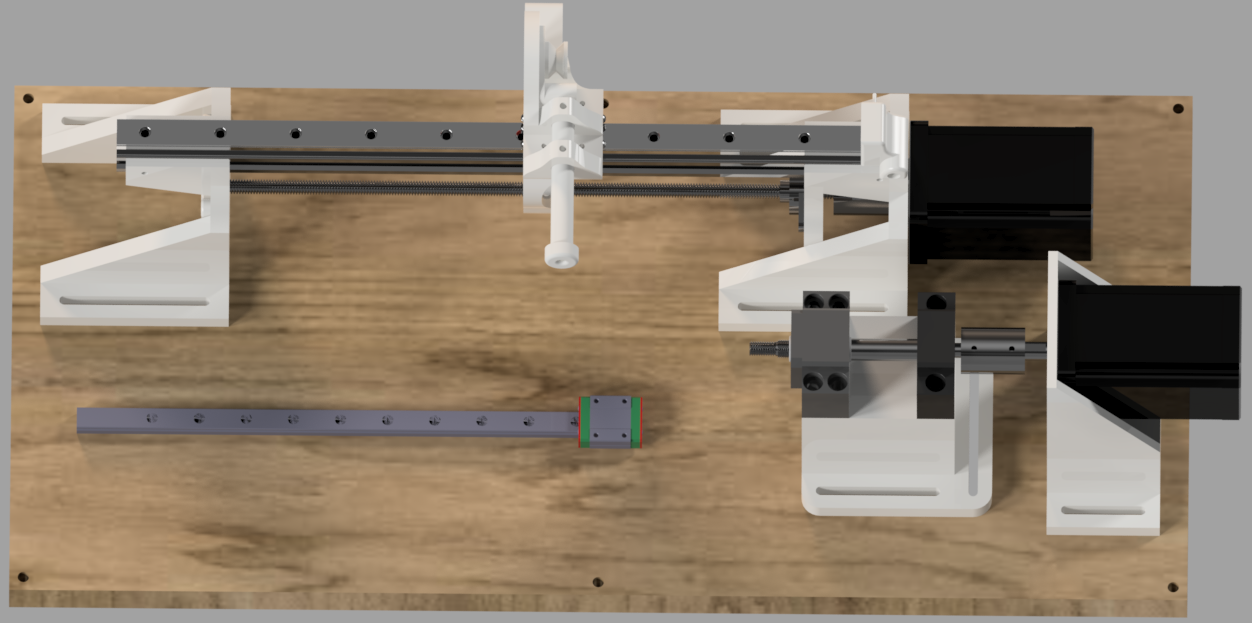
\includegraphics[width=0.55\textwidth]{./winder_render.png}
\end{wrapfigure}

Aufgeteilt ist das Projekt in zwei mechanische Untersyteme, das Drahtspannsystem und der Winder.
Beide Systeme wurden mit 3D-Druck-Teilen aus PETG und Frästeilen aus MDF gebaut und mithilfe unterschiedlicher Schraubsysteme verbunden. Mit Ausnahme der Kaufteile und des Aufnahmewelle, welcher aus hochfestem Stahl passgenau gedreht wurde.



Der Winder besteht aus einer reinen Drehachsen, sowie einem Lineartisch mit gekoppelter Trapetzspindel. Beide Achsen werden jeweils durch einen Steppermotor bewegt. Für die Spulenwicklung, wird der Spulenkörper am Linksgewinde der Aufnahmewelle befestigt und die Achse vom Motor im Uhrzeigersinn gedreht. Die Trapetzspindel kann hingegen in beide Richtungen gedreht werden, bzw. der Lineartisch in beide Richtungen fahren, wodurch die Position des, durch den am Tisch befestigten Aufnahmedorn laufenden, Drahtes, relativ zum Spulenkörper, verändert werden kann. Des Weiteren ist am Lineartisch ein Rotary-Encoder verbaut, sowie ein Gleitlager zur Drahtführung. Sowohl die Gleitlagerhalterung nahe dem Encoder, als auch der Aufnahmedorn, enthalten im Inneren einen Einsatz aus Teflon, um die Reibung zwischen Draht und Führung klein zu halten und Abreibung der Drahtisolation zu vermeiden.

% \begin{figure}[H]
%     \centering
%     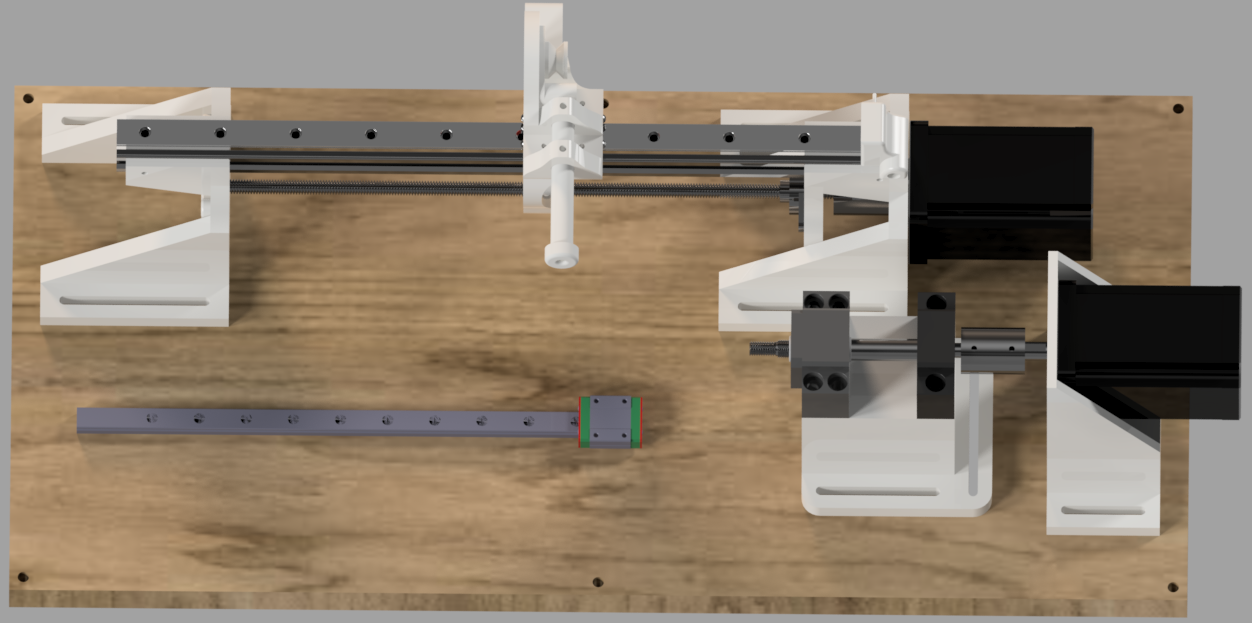
\includegraphics[width=0.25\textwidth]{./winder_render.png}
%     \caption{a nice plot}
%     \label{fig:winder_render}
% \end{figure}

\begin{wrapfigure}{l}{0.30\textwidth}
    \centering
    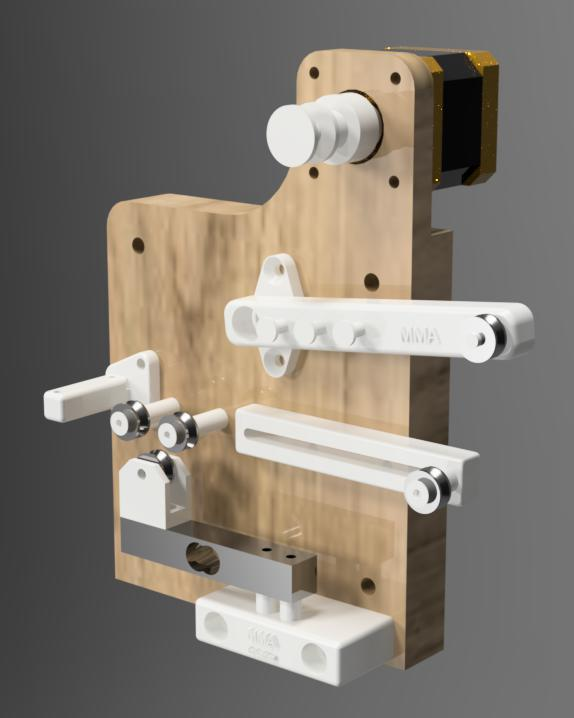
\includegraphics[width=0.30\textwidth]{./spannplatte_render.jpg}
\end{wrapfigure}

Um einen gleimäßige Wicklung zu gewährleisten, muss die Drahtspannung einstellbar sein und von dieser Idealspannung nur in einem kleinen/bekannten Intervall abweichen. Hierzu wird die Rückstellkraft die auf den Draht wirkt durch zwei Schrauben, welche zwei mit Filz beklebte Platten zusammendrückt, eingestellt. Der Draht wird anschließend durch drei Kugellager geführt, wobei das zweite auf einer Wägezelle montiert ist und die Positionierung so gewählt ist, dass ein- und auslaufender Draht, am Kugellager der Wägezelle, ca. einen Winkel von 180° einschließen. Danach wird der Draht über ein weiteres Kugellager, montiert auf einer, mittels Langloch arritierbaren, Leiste, geführt. Von dort aus läuft er über das letzte Lager, welches am Tänzerarm befestigt ist. Dieser Arm ist kugelgelagert und ca. in der Mitte mit einer Feder verbunden. An dieser Feder ist an ihrem anderen Ende eine Schnur befestigt, welche durch einen Steppermotor aufgewickelt werden kann, um so die Feder zu spannen. Der bewegliche Arm kann somit dynamisch auf Drahtspannugsänderungen reagieren.

    %     \section{Sensoren und Akktoren}
\label{sec:Sensoren_Akktoren}

\begin{itemize}
    \item  Bitte keine Copy+Paste Texte vom Hersteller in Text oder Präsentation
    \item  Kurz und knackig, was kann der Sensor
    \item  Was ist das physikalische Messprinzip
    \item  Sensor/Aktor Kalibrierung
        \begin{itemize}
            \item Wie haben Sie gewährleistet, dass der Sensor richtig misst?
            \item Was ist ihr Normativ?
            \item Wie hoch ist die Standardabweichung des Sensors im Ruhezustand mit/ohne 
            System?
        \end{itemize}    
\end{itemize}
    %     \section{Messablauf}
\label{sec:Messablauf}

% Wie läuft die Messung ab? (Ereignis/Kontinuierlich ect.)
% Was für eine Messprozedur wird verwendet?


Das zuwickelnde Medium (Faden, Draht, etc.) wird durch das Spannsystem und die Maschine eingeführt und am Spulenkörperbefestigt. Die Maschine wird, mittels Commandlinebefehlen im Userinterface (UI), an ihre Startposition gefahren. Danach wird der Befehl zum Start des Kalibrationsscriptes gegeben, woraufhin das Programm einen zum tarieren der Wägezelle, sowie zum Messen eines Referenzgewichtes, auffordert. Danach kann der Befehl zum Start des Windingscriptes gesendet werden. Dieses Starten die Datenübertragung über die Serielleschnittstelle an den Computer, danach beginnt der Wickelprozess. Bis zur Beendigung der Wicklung werden kontinuierlich Messdaten an den Computerübertragen. Für den genauen technischen Ablauf der Messung, siehe \autoref{sec:Messschleife}. 

Anmerken wie genau das mit der Kalibration der Wägezelle war, bzw. da wir ja nur an relativ Werten interessiert sind, der schwankende Offset irrelevant ist (z.B. wegen Temperatur).
    %     \section{Messschleife}
\label{sec:Messschleife}

Kern der Messschleife ist die Step-Impuls gebende ISR (Interrupt Service Routine) der Enceladus Software.
Diese ISR wird vom 16 bit Hardware Timer 1 je nach Motorgeschwindigkeit in fixen Zeitabständen ausgelöst.
Die Zeitabstände $\Delta t_{ISR}$ sind dabei die Inverse Step-Impuls Frequenz.
Die zweite zeitliche Limitierung der Messschleife ist die Messdauer des HX711 Chips.
Dieser benötigt $\Delta t_{HX711}$ = 12.5 \si{\milli\second} für eine Messung der Wägezelle.
Da $\Delta t_{HX711}$ im Vergleich zu $\Delta t_{ISR}$ konstant ist, wurde dies als Messintervall gewählt.
Um dies zu erreichen wird in der ISR die Funktion \verb|loadcell.is_ready()| abgefragt, welche nur abfragt ob der HX711 DT pin auf HIGH steht.
Ist dies der Fall, wird der aktuelle Wägezellen Messwert, die Step-Positionen von Haupt und Nebenachse und die aktuelle Zeit mit \verb|millis()| über die Serielle Schnittstelle ohne jegliche Verarbeitung an den PC gesendet.
Dies führte aber zu einigen Limitierungen die durch Zeitdruck nichtmehr umgehbar waren.
Erstens führte das, zu einer maximal möglichen Motordrehzahl von 0.8 U/s, da bei schnelleren Drehzahlen $\Delta t_{HX711} > \Delta t_{ISR}$ war und dadurch Step-Impulse dadurch nicht mehr mit konstanter Frequenz an den Motor gesendet wurden.
Zweitens wird der Wert der \verb|millis()| Funktion während der ISR nicht Aktualisiert, somit entsteht eine Varianz im Messdaten Intervall $\Delta t_{mess}$ = 11 - 13 \si{\milli\second}.


    %     \section{Code}
\label{sec:Code}
    %     \section{Messdaten}
\label{sec:Messdaten}

Für die Durchführung der Experimente wurden zwei Zylinder mit gleicher Höhe $h=50~\si{\milli\metre}$, aber unterschiedlicher Grundfläche, als Spulenkörper verwendet. Die Grundfläche der einen Spule ($SP_K$) entspricht einem Kreis mit Radius $r=10~\si{\milli\metre}$, die der zweiten Spule einem Quadrat ($SP_Q$) mit Seitenlänge $s=20~\si{\milli\metre}$. Die Experimente werden in \autoref{sec:Auswertung} näher ausgeführt. Zur beispielhaften Darstellung der Rohdaten ist hier der, absichtlich herbeigeführte, Abriss des Drahtes während einer Wickeloperation dargestellt.

% \begin{figure}[H]
%     \centering
%     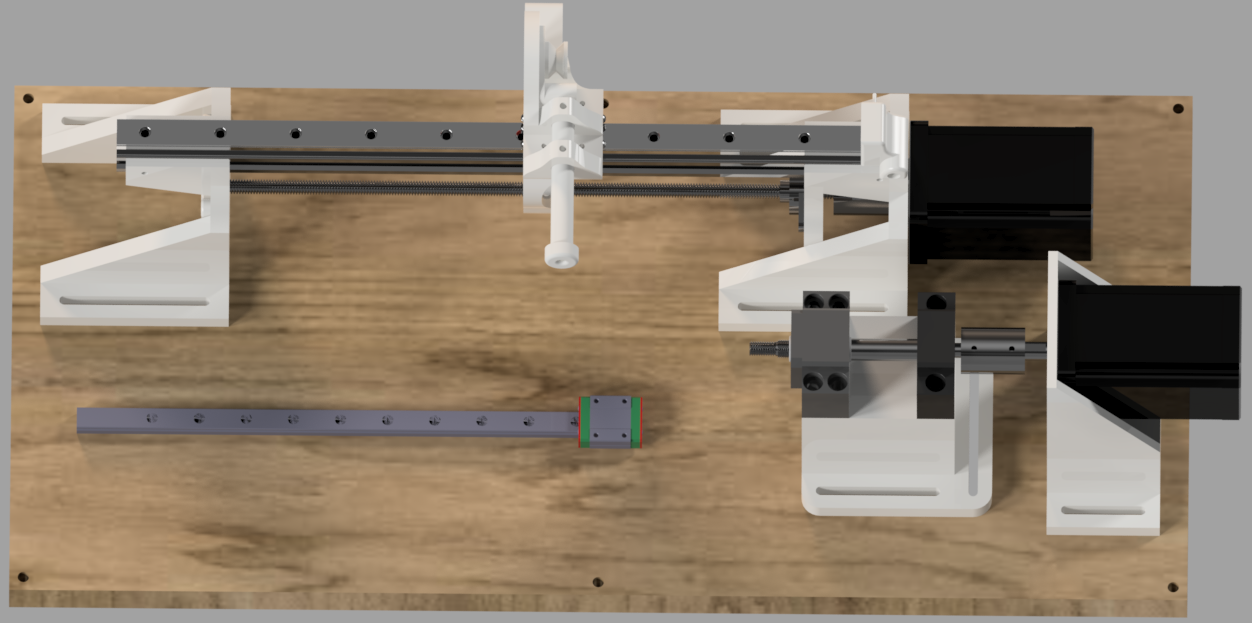
\includegraphics[width=0.25\textwidth]{./winder_render.png}
%     \caption{a nice plot}
%     \label{fig:winder_render}
% % \end{figure}
% \begin{wrapfigure}{l}{0.35\textwidth}
%     \centering
%     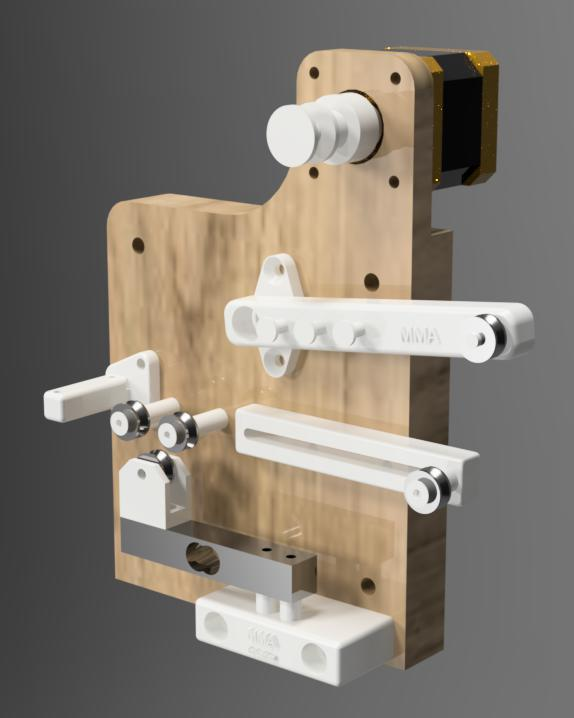
\includegraphics[width=0.35\textwidth]{./spannplatte_render.jpg}
% \end{wrapfigure}
    %     \section{Auswertung}
\label{sec:Auswertung}

Wurde im Folgenden ein Versuch ohne Dancerarm durchgeführt, so wurde der Draht direkt über das Kugellager der darunter liegenden Leiste geführt. Des weiteren gilt für alle folgenden Graphiken, dass die Unsicherheitsbalken stets die einfache Standardabweichung angebegen.\newline
Wickelt man die selbe Wicklung, auf der Spule $SP_K$, zweimal mit unterschiedlicher Geschwindigkeit, so wird der, bereits in \autoref{sec:Physikalisches Modell} erwähnte, Effekt einer geschwindigkeitsabhängigen Drahtspannung , bzw. Rückstellkraft $F_R$ sichtbar. Der Versuch wurde je einmal mit Dancerarm und einmal ohne Dancerarm durchgeführt.

\begin{figure}[H]
    \centering
    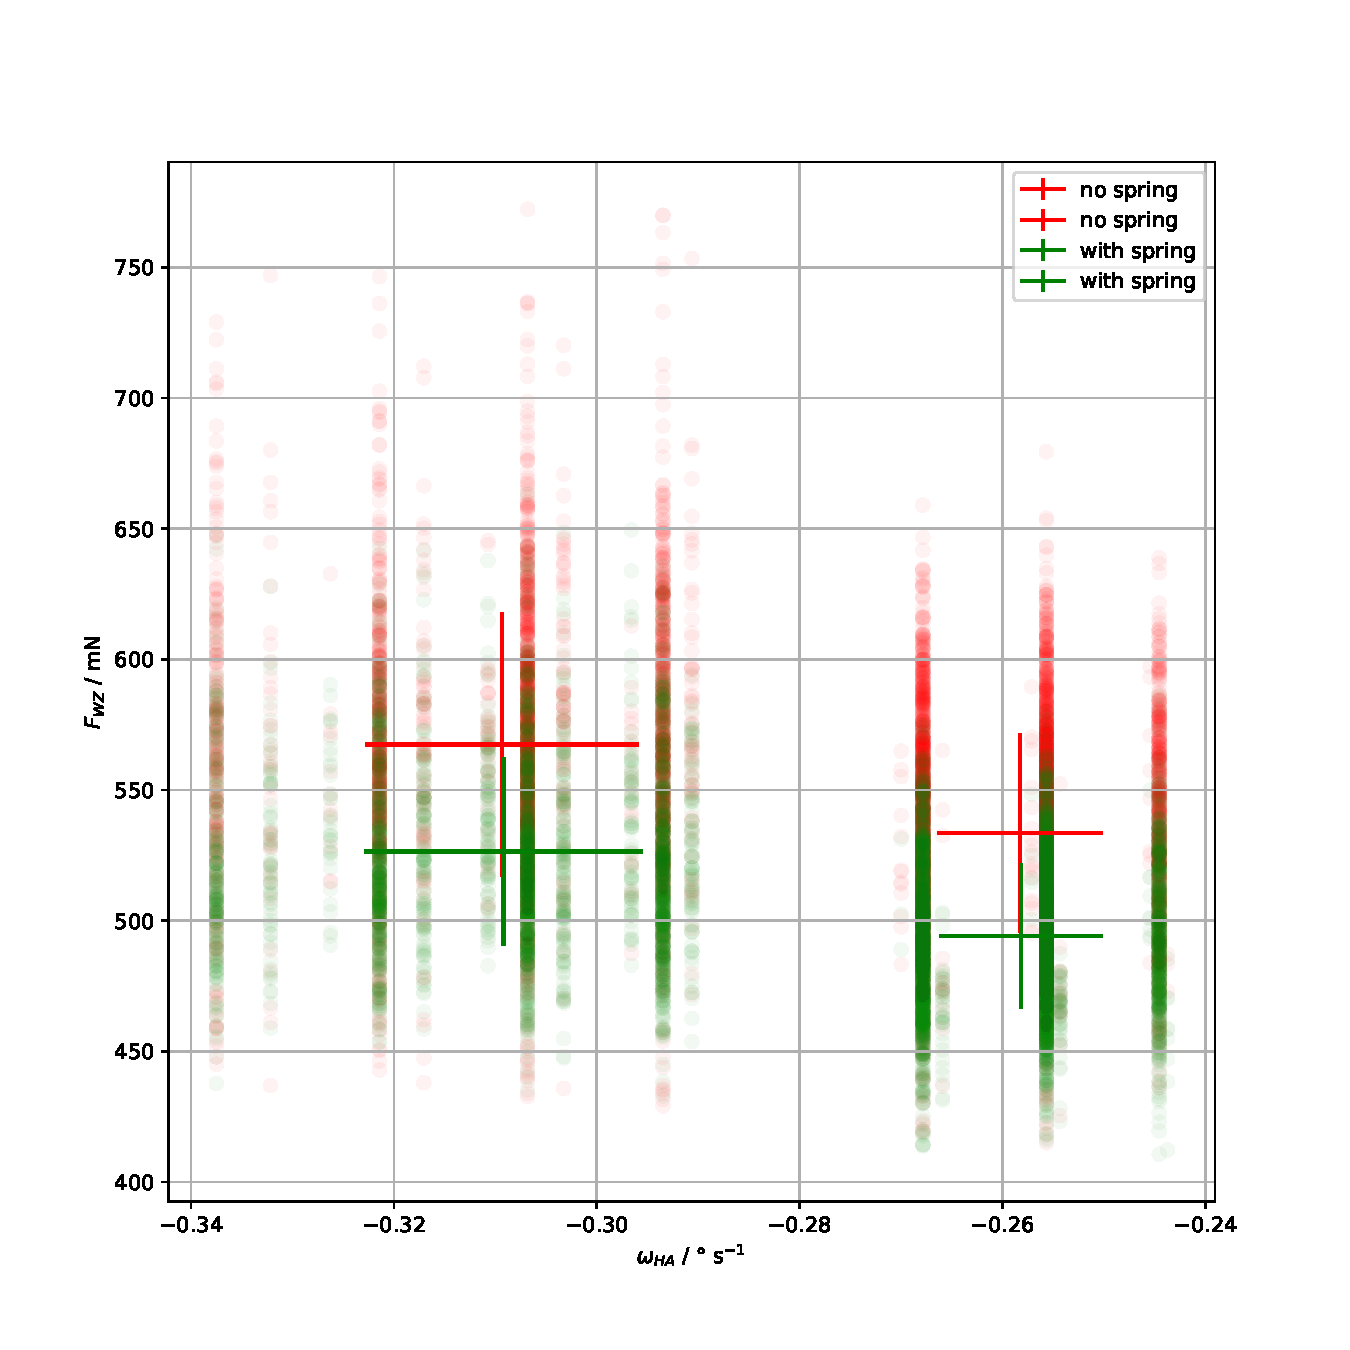
\includegraphics[width=0.9\textwidth]{./const_speed.pdf}
    \caption{Darstellung der an der Wägezelle gemessenen Kraft während einer Wickelphase mit vorgegebener, konstanter Geschwindigkeit, $F_{WZ}$ in Abhängigkeit von der Winkelgeschwindigkeit der Hauptachse $\omega_{HA}$. Die, mit Unsicherheitsbalken versehenen, vier Datenpunkte beschreiben jeweils das arithmetische Mittel des angegeben Größe.}
    \label{fig:plot_const_speed}
\end{figure}


Eine mögliche Erklärung für die, in siehe \autoref{fig:plot_const_speed} ersichtliche, Geschwindigkeitsabhängigkeit der Drahtspannungskraft $\tau(v)$, bzw. Rückstellkraft $F_R(v)$, wäre, dass sich die Reibung an Filz !!!!!!!!!!!!! \newline
% #TODO:Schreiben
% Einfügen erklärung filz wie gas reibung und Erklärung kugellageröl viskosität


Für den nächsten Versuch wurden die selbe Wicklung, bei gleichbleibenden Wickelparametern, einmal mit Dancerarm und einmal ohne, je für beide Spulenkörper, durchgeführt. Da die Zeit zwischen zwei Messwerten nicht konstant ist, sondern leicht schwankt (für Erklärung siehe \autoref{sec:Messschleife}), wurden die Daten Interpoliert, um äquidistante Messwertschritte zu erhalten. Danach wurde jeweils eine Fast-Fourier-Transformation $FFT$ durchgeführt und das Ergebnis in \autoref{fig:ffts} dargestellt.

\begin{figure}[H]
    \centering
    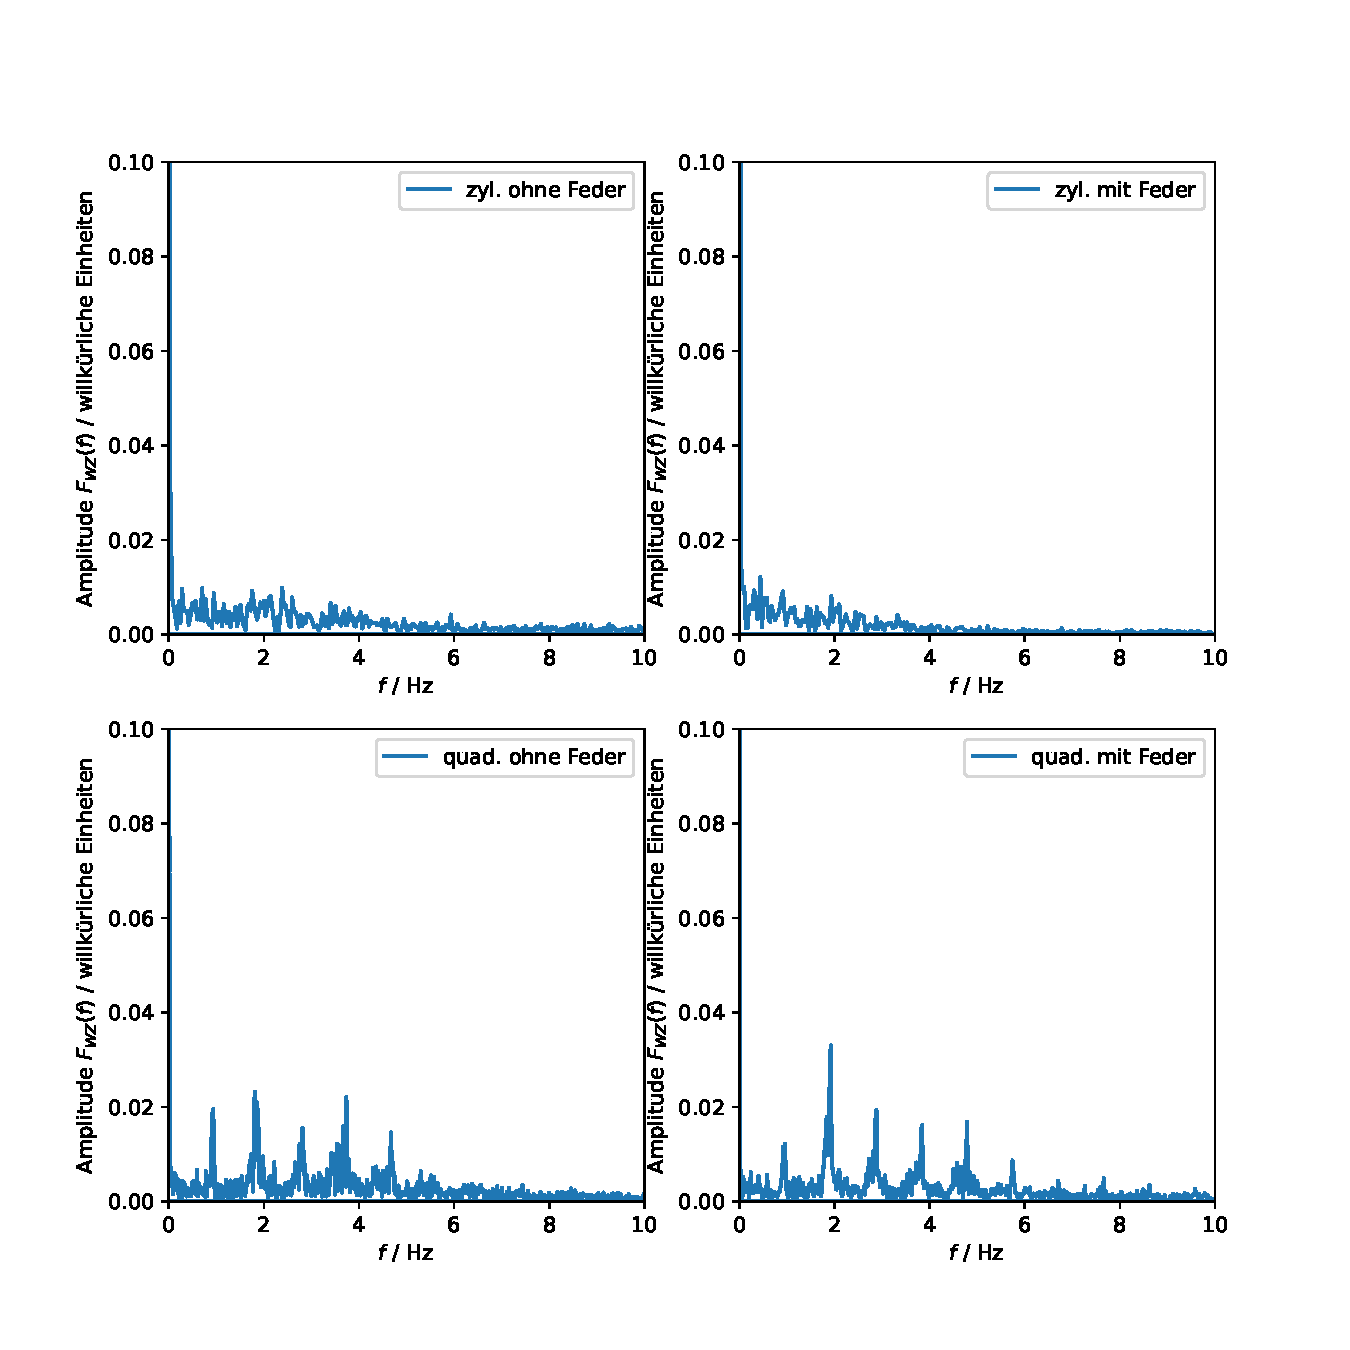
\includegraphics[width=0.9\textwidth]{./ffts.pdf}
    \caption{Darstellung der $FFTs$ für beide Spulenkörper, je einmal ohne Dancerarm und einmal mit Arm}
    \label{fig:ffts}
\end{figure}

Betrachtet man die zwei, $SP_K$, zugehörigen Graphen, in \autoref{fig:ffts}, so sieht man, dass es keinen signifikanten Unterschied gibt wenn der Dancerarm nicht verwendet wird. Der Einfluss der, in \autoref{sec:Physikalisches Modell} vermuteten, abklingenden Schwingung, angeregt durch den Wechsel von Haft- zu Gleitreibung, scheint vergleichsweise wenig Einfluss auf die Schwingung der Drahtspannung zu haben. Sieht man sich hingegen die zwei Graphen von $SP_Q$ an, so fallen sofort die deutlichen Peaks in der $FFT$ auf  welche auf das periodische Schwingen der Drahtspannung hindeuten.

% #TODO: Interpretation der konkreten Frequenzen, nachdem die Frequenz der HA eingefügt wurde
ds\newline

Zur Untersuchung der Start-, bzw. Abbremsphasen eines Wickeldurchganges sind in \autoref{fig:plot_beschleunigung} die zwei Phasen, je für beide Spulentypen dargestellt. Die Messungen wurde jeweils mit der selben Beschleunigung und Endgeschwindigkeit durchgeführt.


\begin{figure}[H]
    \centering
    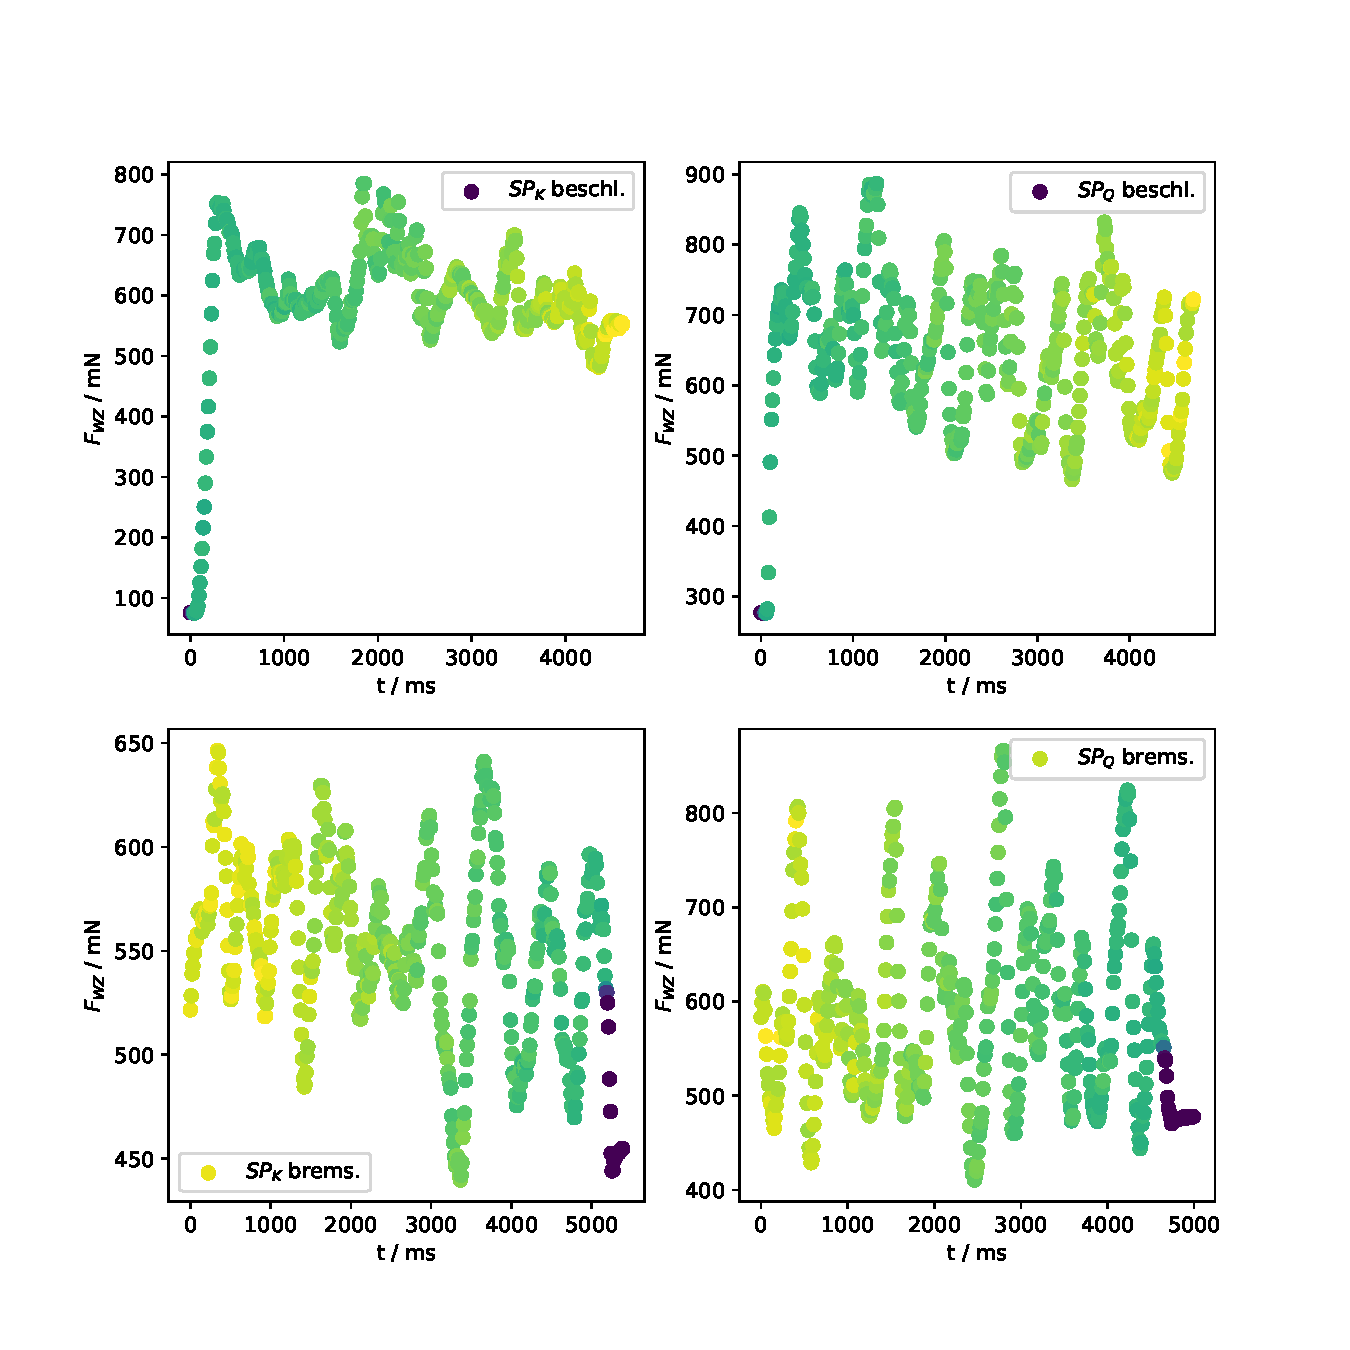
\includegraphics[width=0.9\textwidth]{./besch.pdf}
    \caption{Darstellung der an der Wägezelle gemessenen Kraft $F_{WZ}$ gegen die Zeit $t$. Die Farbcodierung stellt die Geschwindigkeit der HA $\omega_{HA}$, von Gelb (große Geschwindigkeit) bis Lila (kleine Geschwindigkeit), dar. Für alle vier Graphen wurden die selben Wickelparameter verwendet. Die Messungen fanden ohne Dancerarm statt.}
    \label{fig:plot_beschleunigung}
\end{figure}

Sieht man sich die Graphiken der Bremsphasen an, so fällt auf, dass das System stark gedämpft ist. Betrachtet man die lilafärbigen Teile des Datensatzes, so sieht man nur einen relativen kleinen trägheitsbedingten Ausschwung der Kraft unter die anschließende Ruhelage. Die Filzklemme scheint also ihre im Modell (siehe \autoref{sec:Physikalisches Modell}) angedachte Funktion gut zu erfüllen. Im Bezug auf die Beschleunigungsphasen ist anzumerken, dass das die Kraft sehr schnell anfängt um einen Wert herum zu schwanken, obwohl die Beschleunigungsphase immer noch anhält. Dies wurde von uns ebenfalls nicht erwartet, da hier mit einer konstanten Beschleunigung gearbeitet wurde.  




    %     \section{Conclusio}
\label{sec:Conclusio}

Wie sich herausgestellt
% Wie sich experimentell allerdings herausstellte, weißt die Drahtspannung eine Geschwindigkeitsabhängigkeit auf. Bei höherer Aufwickelgeschwindigkeit liegt auch eine höhere Drahtspannung vor. Dies lässt widerspricht dem oben beschrieben Modell und deutet auf eine geschwindigkeitsabhängige Rückstellkraft $F_{R}(t)$ hin, auf welche näher in \autoref{sec:Auswertung} eingegangen wird.

geschwindigkeitsabhängigkeit 

    % \end{multicols}


\section{Aufgabenstellung}
\label{sec:Aufgabenstellung}
\section{Physikalisches Modell}
\label{sec:Physikalisches Modell}

\begin{itemize}
    \item Was für ein System wollen Sie betrachten, was für Gesetzmäßigkeiten liegen vor?
    \item Welche Formeln sollten gültig sein?
    \item Wie könnte das System modelliert werden?
    \item Welche möglichen Störgrößen würden Sie erwarten?
\end{itemize}


\section{Hardware}
\label{sec:Hardware}



\begin{itemize}
    \item HX711
    \item Arduino UNO (ATMEGA328p)
    \item TMC2209 Driver
    \item Schaltplan
    \item Wägezelle
    \item Steppermotor ACT 24HS5430D8L2
    full step $1,8 \pm 5$ per step;
    3 A/phase;
    2,4 V;
    150 N.cm Haltemoment;
    350 $g \cdot cm^2$ Drehmoment;
    \item Netzteil
    \item Stepdownconverter
\end{itemize}


% \item  Bitte keine Copy+Paste Texte vom Hersteller in Text oder Präsentation
% Kurz und knackig, was kann der Sensor
% Was ist das physikalische Messprinzip
% Sensor/Aktor Kalibrierung
%     Wie haben Sie gewährleistet, dass der Sensor richtig misst?
%     Was ist ihr Normativ?
%     Wie hoch ist die Standardabweichung des Sensors im Ruhezustand mit/ohne System?









\section{Mechanik}
\label{sec:Mechanik}

% #TODO: Abschnitt kontrollieren
% #TODO: Abschnitt final absegnen (erst wenn alles andere auch fertig ist!)

% #TODO: Bilder mit Pfeilen und Text versehen

% Wie ist das System realisiert?

\begin{wrapfigure}{r}{0.55\textwidth}
    \centering
    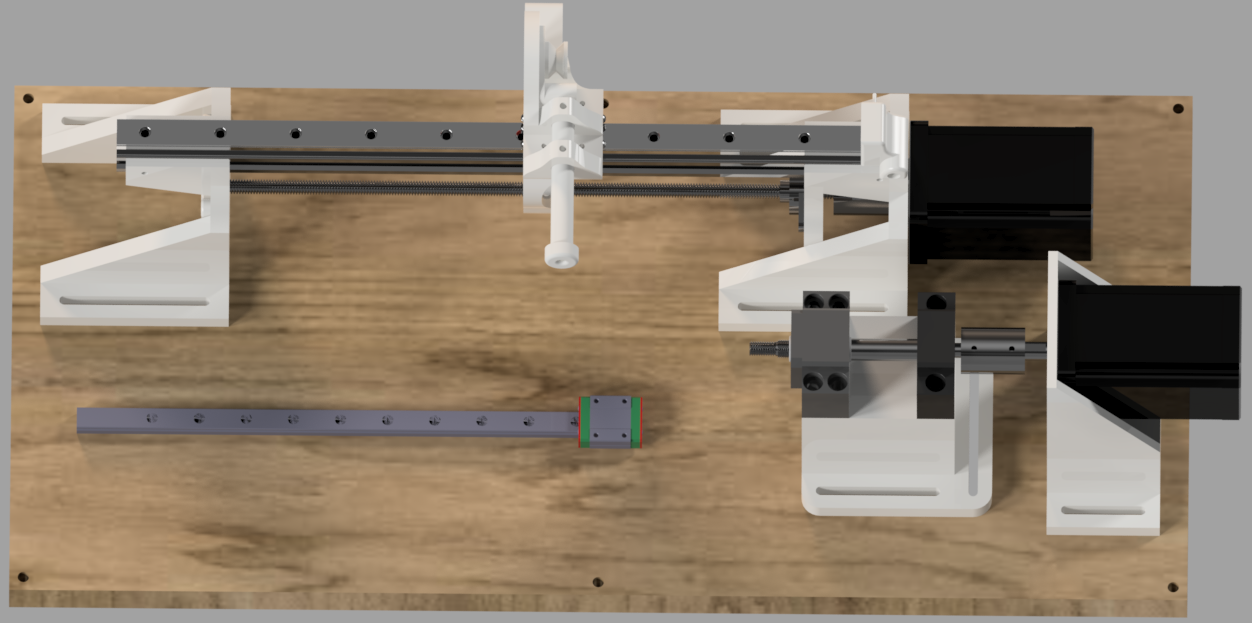
\includegraphics[width=0.55\textwidth]{./winder_render.png}
\end{wrapfigure}

Aufgeteilt ist das Projekt in zwei mechanische Untersyteme, das Drahtspannsystem und der Winder.
Beide Systeme wurden mit 3D-Druck-Teilen aus PETG und Frästeilen aus MDF gebaut und mithilfe unterschiedlicher Schraubsysteme verbunden. Mit Ausnahme der Kaufteile und des Aufnahmewelle, welcher aus hochfestem Stahl passgenau gedreht wurde.



Der Winder besteht aus einer reinen Drehachsen, sowie einem Lineartisch mit gekoppelter Trapetzspindel. Beide Achsen werden jeweils durch einen Steppermotor bewegt. Für die Spulenwicklung, wird der Spulenkörper am Linksgewinde der Aufnahmewelle befestigt und die Achse vom Motor im Uhrzeigersinn gedreht. Die Trapetzspindel kann hingegen in beide Richtungen gedreht werden, bzw. der Lineartisch in beide Richtungen fahren, wodurch die Position des, durch den am Tisch befestigten Aufnahmedorn laufenden, Drahtes, relativ zum Spulenkörper, verändert werden kann. Des Weiteren ist am Lineartisch ein Rotary-Encoder verbaut, sowie ein Gleitlager zur Drahtführung. Sowohl die Gleitlagerhalterung nahe dem Encoder, als auch der Aufnahmedorn, enthalten im Inneren einen Einsatz aus Teflon, um die Reibung zwischen Draht und Führung klein zu halten und Abreibung der Drahtisolation zu vermeiden.

% \begin{figure}[H]
%     \centering
%     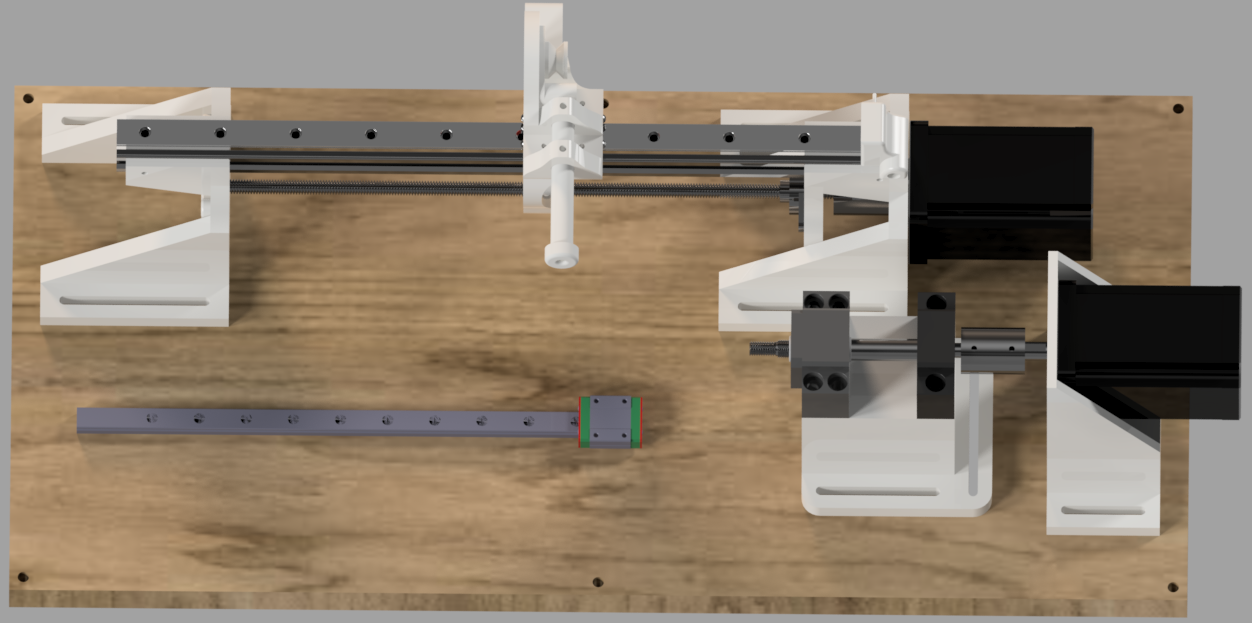
\includegraphics[width=0.25\textwidth]{./winder_render.png}
%     \caption{a nice plot}
%     \label{fig:winder_render}
% \end{figure}

\begin{wrapfigure}{l}{0.30\textwidth}
    \centering
    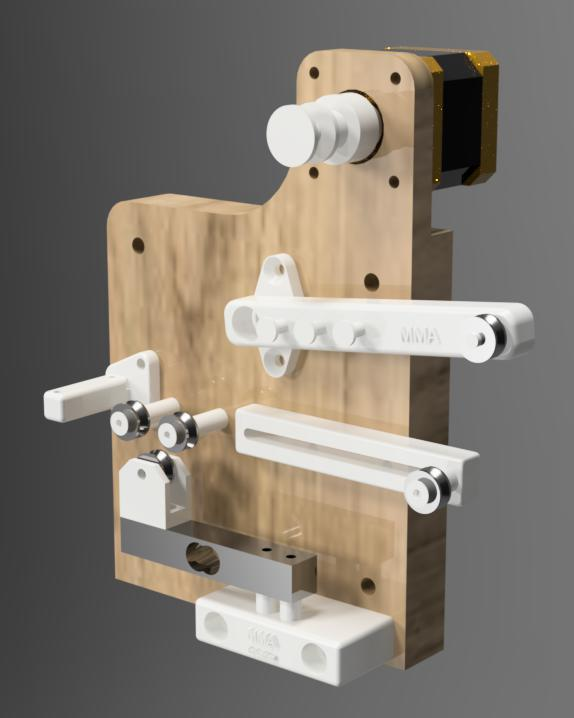
\includegraphics[width=0.30\textwidth]{./spannplatte_render.jpg}
\end{wrapfigure}

Um einen gleimäßige Wicklung zu gewährleisten, muss die Drahtspannung einstellbar sein und von dieser Idealspannung nur in einem kleinen/bekannten Intervall abweichen. Hierzu wird die Rückstellkraft die auf den Draht wirkt durch zwei Schrauben, welche zwei mit Filz beklebte Platten zusammendrückt, eingestellt. Der Draht wird anschließend durch drei Kugellager geführt, wobei das zweite auf einer Wägezelle montiert ist und die Positionierung so gewählt ist, dass ein- und auslaufender Draht, am Kugellager der Wägezelle, ca. einen Winkel von 180° einschließen. Danach wird der Draht über ein weiteres Kugellager, montiert auf einer, mittels Langloch arritierbaren, Leiste, geführt. Von dort aus läuft er über das letzte Lager, welches am Tänzerarm befestigt ist. Dieser Arm ist kugelgelagert und ca. in der Mitte mit einer Feder verbunden. An dieser Feder ist an ihrem anderen Ende eine Schnur befestigt, welche durch einen Steppermotor aufgewickelt werden kann, um so die Feder zu spannen. Der bewegliche Arm kann somit dynamisch auf Drahtspannugsänderungen reagieren.

\section{Sensoren und Akktoren}
\label{sec:Sensoren_Akktoren}

\begin{itemize}
    \item  Bitte keine Copy+Paste Texte vom Hersteller in Text oder Präsentation
    \item  Kurz und knackig, was kann der Sensor
    \item  Was ist das physikalische Messprinzip
    \item  Sensor/Aktor Kalibrierung
        \begin{itemize}
            \item Wie haben Sie gewährleistet, dass der Sensor richtig misst?
            \item Was ist ihr Normativ?
            \item Wie hoch ist die Standardabweichung des Sensors im Ruhezustand mit/ohne 
            System?
        \end{itemize}    
\end{itemize}
\section{Messablauf}
\label{sec:Messablauf}

% Wie läuft die Messung ab? (Ereignis/Kontinuierlich ect.)
% Was für eine Messprozedur wird verwendet?


Das zuwickelnde Medium (Faden, Draht, etc.) wird durch das Spannsystem und die Maschine eingeführt und am Spulenkörperbefestigt. Die Maschine wird, mittels Commandlinebefehlen im Userinterface (UI), an ihre Startposition gefahren. Danach wird der Befehl zum Start des Kalibrationsscriptes gegeben, woraufhin das Programm einen zum tarieren der Wägezelle, sowie zum Messen eines Referenzgewichtes, auffordert. Danach kann der Befehl zum Start des Windingscriptes gesendet werden. Dieses Starten die Datenübertragung über die Serielleschnittstelle an den Computer, danach beginnt der Wickelprozess. Bis zur Beendigung der Wicklung werden kontinuierlich Messdaten an den Computerübertragen. Für den genauen technischen Ablauf der Messung, siehe \autoref{sec:Messschleife}. 

Anmerken wie genau das mit der Kalibration der Wägezelle war, bzw. da wir ja nur an relativ Werten interessiert sind, der schwankende Offset irrelevant ist (z.B. wegen Temperatur).
\section{Messschleife}
\label{sec:Messschleife}

Kern der Messschleife ist die Step-Impuls gebende ISR (Interrupt Service Routine) der Enceladus Software.
Diese ISR wird vom 16 bit Hardware Timer 1 je nach Motorgeschwindigkeit in fixen Zeitabständen ausgelöst.
Die Zeitabstände $\Delta t_{ISR}$ sind dabei die Inverse Step-Impuls Frequenz.
Die zweite zeitliche Limitierung der Messschleife ist die Messdauer des HX711 Chips.
Dieser benötigt $\Delta t_{HX711}$ = 12.5 \si{\milli\second} für eine Messung der Wägezelle.
Da $\Delta t_{HX711}$ im Vergleich zu $\Delta t_{ISR}$ konstant ist, wurde dies als Messintervall gewählt.
Um dies zu erreichen wird in der ISR die Funktion \verb|loadcell.is_ready()| abgefragt, welche nur abfragt ob der HX711 DT pin auf HIGH steht.
Ist dies der Fall, wird der aktuelle Wägezellen Messwert, die Step-Positionen von Haupt und Nebenachse und die aktuelle Zeit mit \verb|millis()| über die Serielle Schnittstelle ohne jegliche Verarbeitung an den PC gesendet.
Dies führte aber zu einigen Limitierungen die durch Zeitdruck nichtmehr umgehbar waren.
Erstens führte das, zu einer maximal möglichen Motordrehzahl von 0.8 U/s, da bei schnelleren Drehzahlen $\Delta t_{HX711} > \Delta t_{ISR}$ war und dadurch Step-Impulse dadurch nicht mehr mit konstanter Frequenz an den Motor gesendet wurden.
Zweitens wird der Wert der \verb|millis()| Funktion während der ISR nicht Aktualisiert, somit entsteht eine Varianz im Messdaten Intervall $\Delta t_{mess}$ = 11 - 13 \si{\milli\second}.


\section{Code}
\label{sec:Code}
\section{Messdaten}
\label{sec:Messdaten}

Für die Durchführung der Experimente wurden zwei Zylinder mit gleicher Höhe $h=50~\si{\milli\metre}$, aber unterschiedlicher Grundfläche, als Spulenkörper verwendet. Die Grundfläche der einen Spule ($SP_K$) entspricht einem Kreis mit Radius $r=10~\si{\milli\metre}$, die der zweiten Spule einem Quadrat ($SP_Q$) mit Seitenlänge $s=20~\si{\milli\metre}$. Die Experimente werden in \autoref{sec:Auswertung} näher ausgeführt. Zur beispielhaften Darstellung der Rohdaten ist hier der, absichtlich herbeigeführte, Abriss des Drahtes während einer Wickeloperation dargestellt.

% \begin{figure}[H]
%     \centering
%     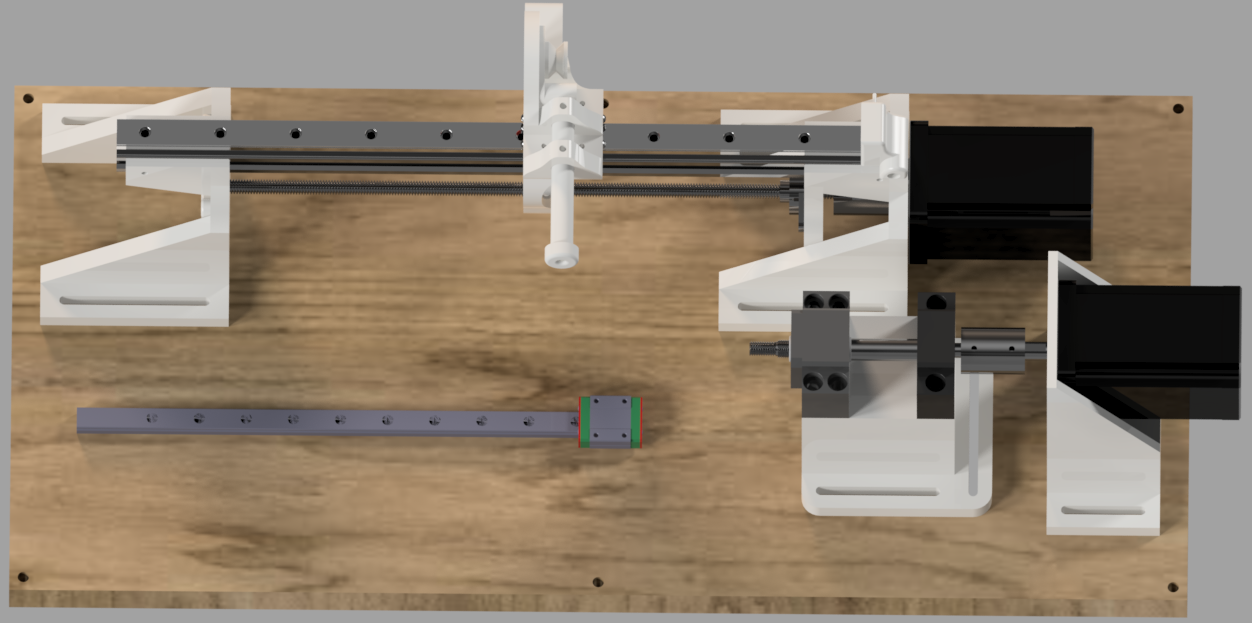
\includegraphics[width=0.25\textwidth]{./winder_render.png}
%     \caption{a nice plot}
%     \label{fig:winder_render}
% % \end{figure}
% \begin{wrapfigure}{l}{0.35\textwidth}
%     \centering
%     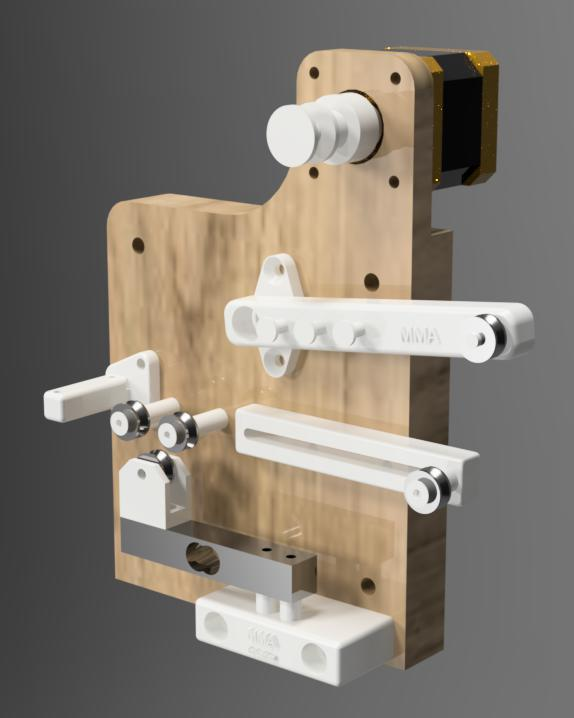
\includegraphics[width=0.35\textwidth]{./spannplatte_render.jpg}
% \end{wrapfigure}
\section{Auswertung}
\label{sec:Auswertung}

Wurde im Folgenden ein Versuch ohne Dancerarm durchgeführt, so wurde der Draht direkt über das Kugellager der darunter liegenden Leiste geführt. Des weiteren gilt für alle folgenden Graphiken, dass die Unsicherheitsbalken stets die einfache Standardabweichung angebegen.\newline
Wickelt man die selbe Wicklung, auf der Spule $SP_K$, zweimal mit unterschiedlicher Geschwindigkeit, so wird der, bereits in \autoref{sec:Physikalisches Modell} erwähnte, Effekt einer geschwindigkeitsabhängigen Drahtspannung , bzw. Rückstellkraft $F_R$ sichtbar. Der Versuch wurde je einmal mit Dancerarm und einmal ohne Dancerarm durchgeführt.

\begin{figure}[H]
    \centering
    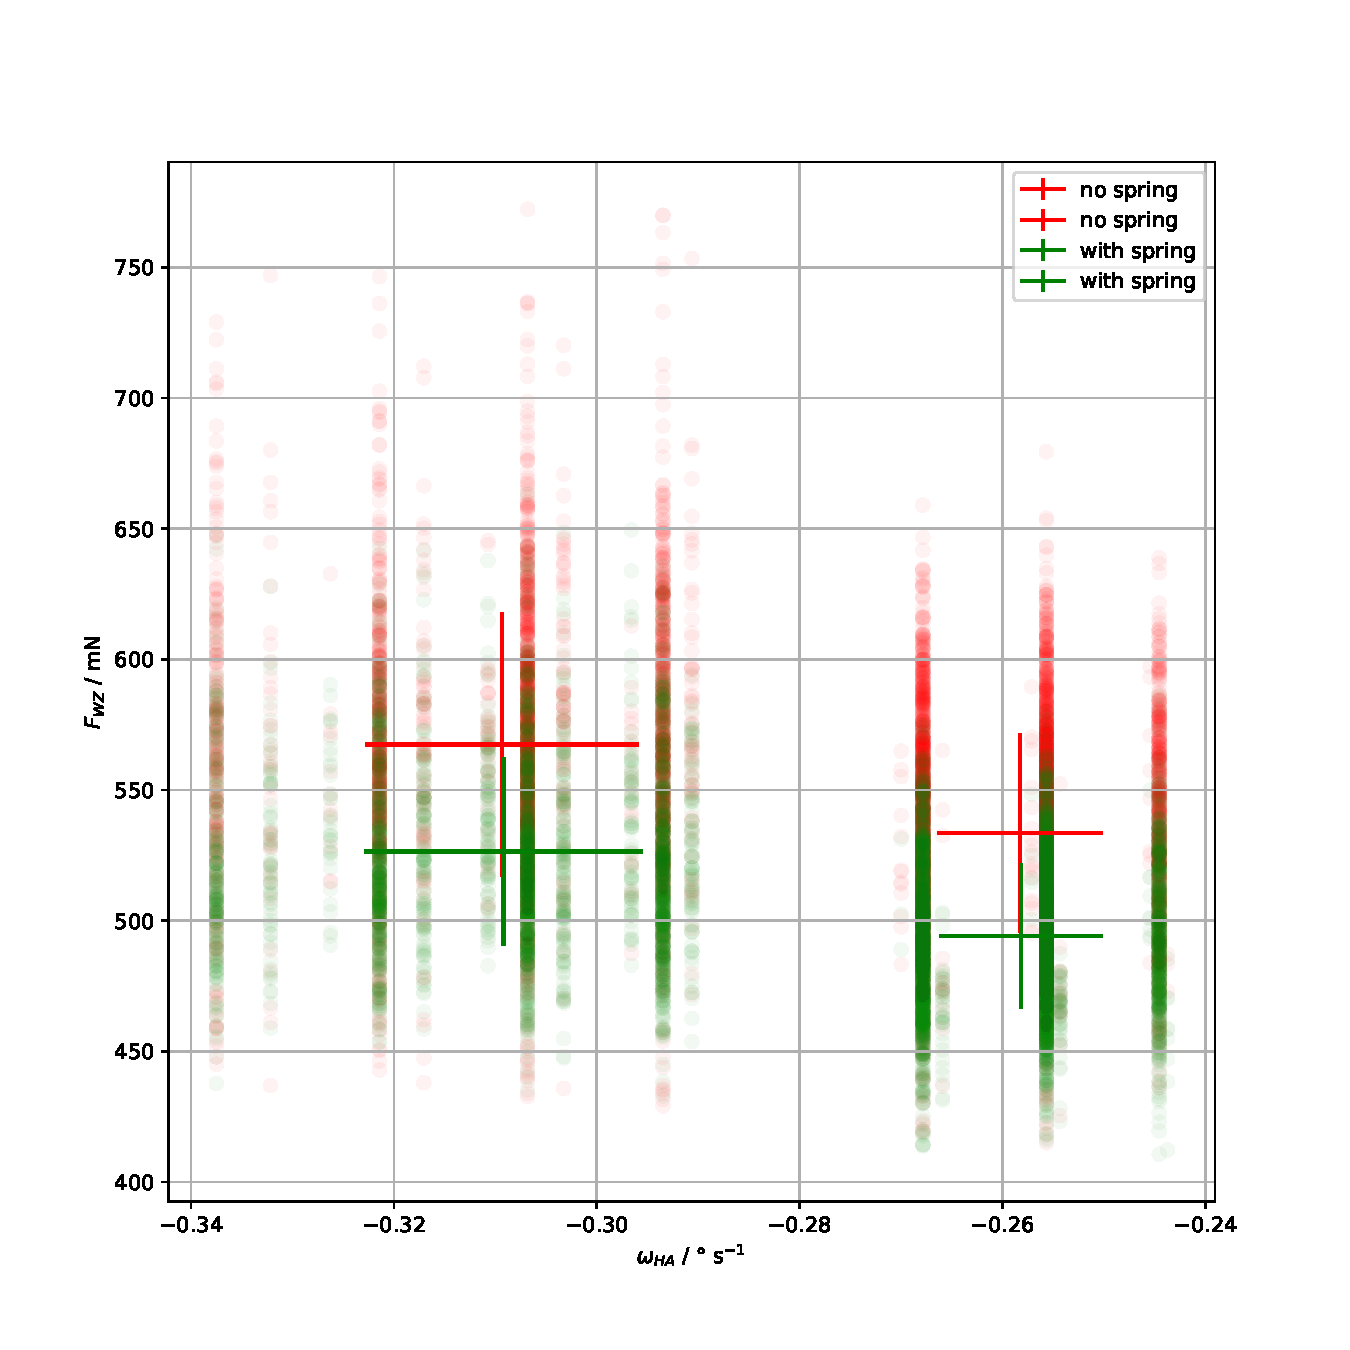
\includegraphics[width=0.9\textwidth]{./const_speed.pdf}
    \caption{Darstellung der an der Wägezelle gemessenen Kraft während einer Wickelphase mit vorgegebener, konstanter Geschwindigkeit, $F_{WZ}$ in Abhängigkeit von der Winkelgeschwindigkeit der Hauptachse $\omega_{HA}$. Die, mit Unsicherheitsbalken versehenen, vier Datenpunkte beschreiben jeweils das arithmetische Mittel des angegeben Größe.}
    \label{fig:plot_const_speed}
\end{figure}


Eine mögliche Erklärung für die, in siehe \autoref{fig:plot_const_speed} ersichtliche, Geschwindigkeitsabhängigkeit der Drahtspannungskraft $\tau(v)$, bzw. Rückstellkraft $F_R(v)$, wäre, dass sich die Reibung an Filz !!!!!!!!!!!!! \newline
% #TODO:Schreiben
% Einfügen erklärung filz wie gas reibung und Erklärung kugellageröl viskosität


Für den nächsten Versuch wurden die selbe Wicklung, bei gleichbleibenden Wickelparametern, einmal mit Dancerarm und einmal ohne, je für beide Spulenkörper, durchgeführt. Da die Zeit zwischen zwei Messwerten nicht konstant ist, sondern leicht schwankt (für Erklärung siehe \autoref{sec:Messschleife}), wurden die Daten Interpoliert, um äquidistante Messwertschritte zu erhalten. Danach wurde jeweils eine Fast-Fourier-Transformation $FFT$ durchgeführt und das Ergebnis in \autoref{fig:ffts} dargestellt.

\begin{figure}[H]
    \centering
    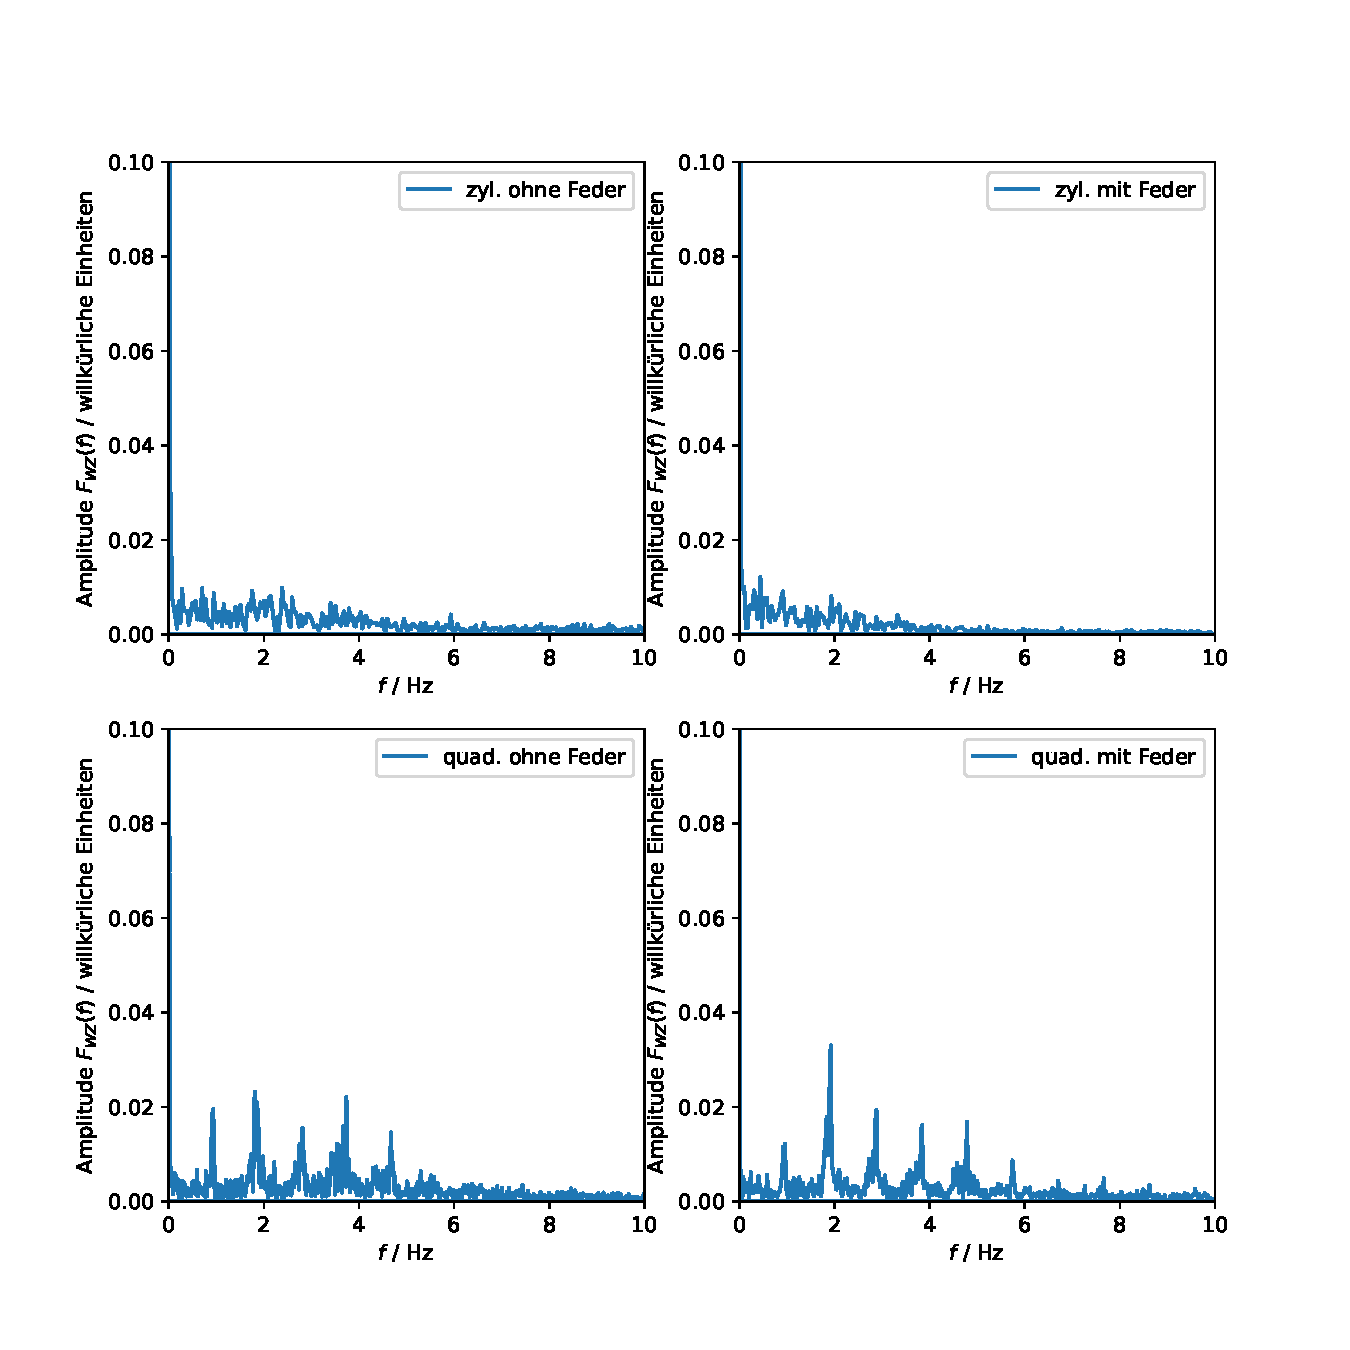
\includegraphics[width=0.9\textwidth]{./ffts.pdf}
    \caption{Darstellung der $FFTs$ für beide Spulenkörper, je einmal ohne Dancerarm und einmal mit Arm}
    \label{fig:ffts}
\end{figure}

Betrachtet man die zwei, $SP_K$, zugehörigen Graphen, in \autoref{fig:ffts}, so sieht man, dass es keinen signifikanten Unterschied gibt wenn der Dancerarm nicht verwendet wird. Der Einfluss der, in \autoref{sec:Physikalisches Modell} vermuteten, abklingenden Schwingung, angeregt durch den Wechsel von Haft- zu Gleitreibung, scheint vergleichsweise wenig Einfluss auf die Schwingung der Drahtspannung zu haben. Sieht man sich hingegen die zwei Graphen von $SP_Q$ an, so fallen sofort die deutlichen Peaks in der $FFT$ auf  welche auf das periodische Schwingen der Drahtspannung hindeuten.

% #TODO: Interpretation der konkreten Frequenzen, nachdem die Frequenz der HA eingefügt wurde
ds\newline

Zur Untersuchung der Start-, bzw. Abbremsphasen eines Wickeldurchganges sind in \autoref{fig:plot_beschleunigung} die zwei Phasen, je für beide Spulentypen dargestellt. Die Messungen wurde jeweils mit der selben Beschleunigung und Endgeschwindigkeit durchgeführt.


\begin{figure}[H]
    \centering
    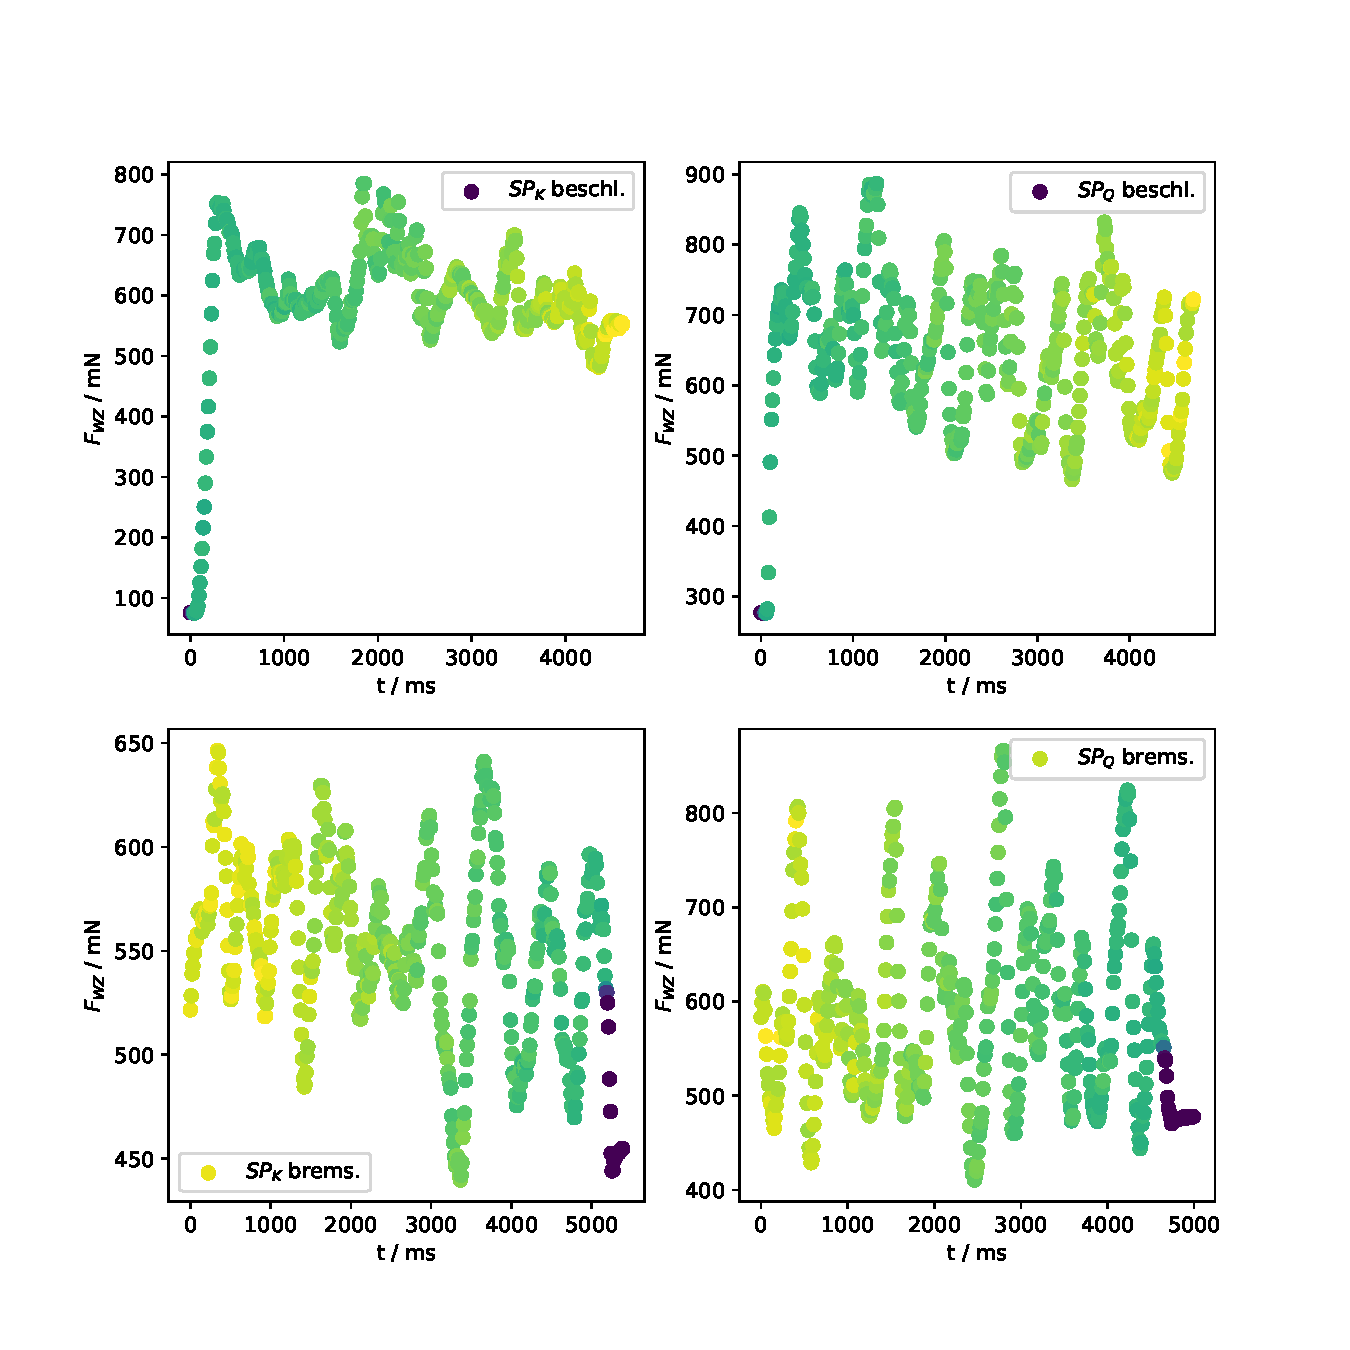
\includegraphics[width=0.9\textwidth]{./besch.pdf}
    \caption{Darstellung der an der Wägezelle gemessenen Kraft $F_{WZ}$ gegen die Zeit $t$. Die Farbcodierung stellt die Geschwindigkeit der HA $\omega_{HA}$, von Gelb (große Geschwindigkeit) bis Lila (kleine Geschwindigkeit), dar. Für alle vier Graphen wurden die selben Wickelparameter verwendet. Die Messungen fanden ohne Dancerarm statt.}
    \label{fig:plot_beschleunigung}
\end{figure}

Sieht man sich die Graphiken der Bremsphasen an, so fällt auf, dass das System stark gedämpft ist. Betrachtet man die lilafärbigen Teile des Datensatzes, so sieht man nur einen relativen kleinen trägheitsbedingten Ausschwung der Kraft unter die anschließende Ruhelage. Die Filzklemme scheint also ihre im Modell (siehe \autoref{sec:Physikalisches Modell}) angedachte Funktion gut zu erfüllen. Im Bezug auf die Beschleunigungsphasen ist anzumerken, dass das die Kraft sehr schnell anfängt um einen Wert herum zu schwanken, obwohl die Beschleunigungsphase immer noch anhält. Dies wurde von uns ebenfalls nicht erwartet, da hier mit einer konstanten Beschleunigung gearbeitet wurde.  




\section{Conclusio}
\label{sec:Conclusio}

Wie sich herausgestellt
% Wie sich experimentell allerdings herausstellte, weißt die Drahtspannung eine Geschwindigkeitsabhängigkeit auf. Bei höherer Aufwickelgeschwindigkeit liegt auch eine höhere Drahtspannung vor. Dies lässt widerspricht dem oben beschrieben Modell und deutet auf eine geschwindigkeitsabhängige Rückstellkraft $F_{R}(t)$ hin, auf welche näher in \autoref{sec:Auswertung} eingegangen wird.

geschwindigkeitsabhängigkeit 

\end{document}